\subsection{Apparatus}
It is possible to measure the values in the equations above. Using simple a cylindrical shell anode, which measures the electrons emitted from the filament as a current, we can measure the current volume density $J$ as the current through the anode, $I_a$ (see Fig. \ref{Electrode}). \\

Using the circuit diagram from Figure \ref{Circuit}, the filament wire is heated and generates thermionic emission of electrons which is measured at the anode. A voltmeter and ammeter measure both the current and voltage for both the filament and the anode.\\

\begin{figure}[H]
\centering
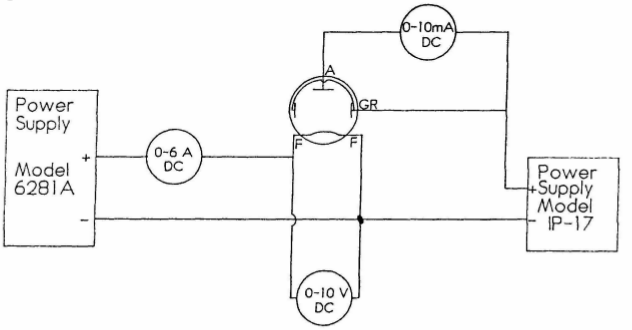
\includegraphics[width=0.8\textwidth]{figures/CircuitDiagram.png}
\caption{Circuit diagram of experimental setup for the detection of thermionic emission.}
\label{Circuit}
\end{figure}

\begin{figure}[H]
\centering
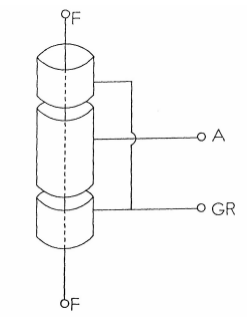
\includegraphics[width=0.3\textwidth]{figures/ElectrodeStructure.png}
\caption{Electrode structure, with filament wire emitting electrons along the axis and coaxial anode and guard rings.}
\label{Electrode}
\end{figure}

\subsection{Experimental Procedure}

\subsubsection{Data Collection}

Our data collection method is based around ramping the current values, and also obtaining a voltage ramp (of $V_a$ for each of the anode current values ($I_a$)). Data points will be collected for Anode Voltages ($V_a$) of 300, 250, 200, 150 \& 100 V at Anode Currents of ($I_a$) of 8.00, 4.00, 0.80 \& 0.40 mA. The steps for doing so are as follows:\\

\begin{steps}
    \item Turn off filament power supply.
    \label{ramp_step_begin}
    
    \item Set the Anode Voltage ($V_a$) to our first value (300 V), this value is verified through the voltmeter connected to the power supply.
    
    \item Turn on filament power supply. 
    
    \item Set the Anode Current ($I_a$) to our first value (8.00 mA) and verify this value through the anode's ammeter.
    
    \item Record the filament Voltage ($I_f$) and Current ($I_f$) by rewiring the ammeter and voltmeter to measure across the filament. These values should stay constant throughout the anode's voltage ramp.
    
    \item Rewire to measure $V_a$ \& $I_a$. 
    
    \item Ramp the $V_a$ down from 300 V to 100 V in 50 V steps. $V_a$ is always set without the filament power supply being on. 
    
    \item Measure $V_a$ and $I_a$ at each step with the filament supply on.
    \label{ramp_step_end}
    
    \item Set the next $I_a$ value. Complete \ref{ramp_step_begin} to \ref{ramp_step_end} with our new $I_a$
    

\end{steps}
